
%%%%%%
%
% $Autor: Manoj Selvaraju $
% $Datum: 2024-01-05 11:15:45Z $
% $Pfad: githubtemplate/Template/report/rename.tex $
% $Version: 4620 $
%
%
% !TeX encoding = utf8
% !TeX root = Rename
% !TeX TXS-program:bibliography = txs:///bibtex
%
%%%%%%




\chapter{Methodology}
\section{KDD Process}
The Knowledge Discovery in Databases (KDD) is a process in data science and analytics focused to discover and make explicit knowledge available in extensive large data sets. \cite{Wings:2024}

The KDD process typically includes several key stages, refer figure ~\ref{fig:KDDProcess}:
\begin{enumerate}
	\item \textbf{Data Selection:} Identifying and gathering relevant data from various sources. In this project, we are gathering our own datasets with three distinct labels.
	
	\item \textbf{Data Preprocessing:} Cleaning and transforming the data to improve its quality. In this project, the preprocessing of the face images includes image resizing and converting to grayscale, reducing complexity to fit to the model. 
	
	\item \textbf{Data Transformation:} The data is transformed to suitable format to focus on key attributes that are significant for analysis. Techniques like normalization, aggregation, and feature extraction are often used. For this prject, the selected images were converted into a suitable dimensions necessary for the machine learning model.
	
	\item \textbf{Data Mining:} The core of KDD, where algorithms are defined, trained and optimized to the prepared data to extract patterns. The MobileNetV2 CNN algorithm is used to for face detection.
	
	\item \textbf{Interpretation/Evaluation:} This step involves analyzing and assessing the discovered patterns to determine their validity and usefulness. Here, Model performance was evaluated using metrics such as F1 score and accuracy
	
	\item \textbf{Knowledge Presentation:} Presenting the discovered knowledge in a way that users can understand using Visualization techniques, reports, or dashboards. Here the results are visualized and deployed to Portenta H7 device.

\end{enumerate}
\begin{comment}
	\begin{figure}[h]
		\centering
		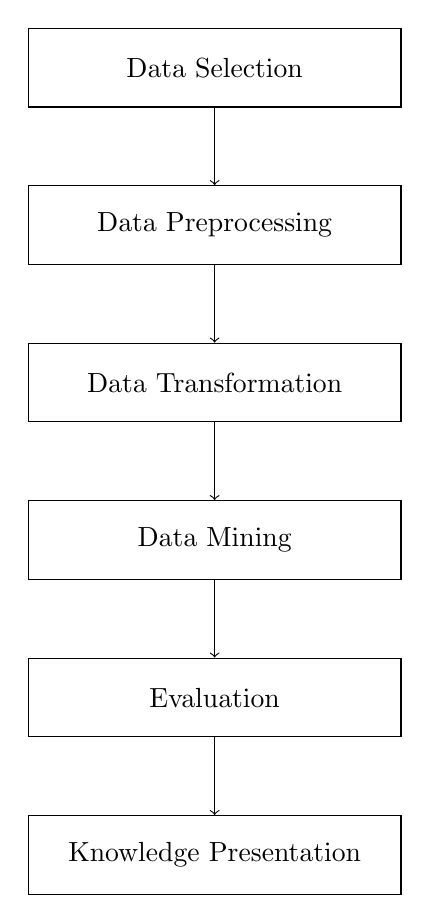
\begin{tikzpicture}[node distance=2cm, auto]
			% Node style
			\tikzstyle{block} = [rectangle, draw=black, text width=4.5cm, text centered, minimum height=1cm]
			
			% Nodes
			\node[block] (selection) {Data Selection};
			\node[block, below of=selection] (preprocessing) {Data Preprocessing};
			\node[block, below of=preprocessing] (transformation) {Data Transformation};
			\node[block, below of=transformation] (mining) {Data Mining};
			\node[block, below of=mining] (evaluation) {Evaluation};
			\node[block, below of=evaluation] (presentation) {Knowledge Presentation};
			
			% Arrows
			\draw[->] (selection) -- (preprocessing);
			\draw[->] (preprocessing) -- (transformation);
			\draw[->] (transformation) -- (mining);
			\draw[->] (mining) -- (evaluation);
			\draw[->] (evaluation) -- (presentation);
			
		\end{tikzpicture}
		\caption{KDD Process}
		\label{fig:KDDProcess}
	\end{figure}
\end{comment}

\begin{figure}
	\begin{center}
		\includegraphics[width=0.7\linewidth]{Images/EdgeImpulse/KDDProcessWings.png}
		\caption{KDD Process}
		\label{fig:KDDProcess}
		\cite{Wings:2024}
	\end{center}
\end{figure}


\section{Justification}

The KDD process was selected for its clear and systematic workflow, ensuring each step from data preparation to deployment is effectively managed. It integrates well with Edge Impulse Studio, simplifying tasks like preprocessing and transformation of images for the model. \\
MobileNetV2, a type of Convolutional Neural Network (CNN) was selected for this project, which introduces inverted residual blocks, which expand the input channels, perform lightweight computations. MobileNetV2’s architecture uses Linear Bottlenecks, which is optimized for extracting features from images, such as facial contours, expressions and unique attributes, even when images are preprocessed to lower dimensions. MobileNetV2 supports INT8 quantization, reducing memory usage and speeding up inference can fit into the 8 MB flash memory of the Portenta H7.